\documentclass{article}
\usepackage{indentfirst}
\usepackage[utf8]{inputenc}
\usepackage[T1]{fontenc}
\usepackage[brazilian]{babel}
\usepackage{lmodern}
\usepackage{graphicx}
\usepackage{float}
\usepackage[]{subfigure}
\usepackage{afterpage}
\usepackage{amsmath}
\usepackage{textcomp,gensymb}
\usepackage{nameref}
\usepackage{accents}
\usepackage{listings}
\usepackage{color,soul}
\usepackage[margin=1in]{geometry}
\usepackage{steinmetz}
\usepackage{xurl}
\usepackage[mathscr]{euscript}




\PassOptionsToPackage{hyphens}{url}\usepackage{hyperref}
\hypersetup{
    breaklinks = true,
}
\urlstyle{same}
\newcommand{\ubar}[1]{\underaccent{\bar}{#1}}
\renewcommand\thesection{\arabic{section}}
\renewcommand\thesubsection{(\alph{subsection})}
\definecolor{dkgreen}{rgb}{0,0.6,0}
\definecolor{gray}{rgb}{0.5,0.5,0.5}
\definecolor{mauve}{rgb}{0.58,0,0.82}
\lstset{
    frame=tb,
    language=Matlab,
    aboveskip=3mm,
    belowskip=3mm,
    showstringspaces=false,
    basicstyle={\small\ttfamily},
    numbers=none,
    numberstyle=\tiny\color{gray},
    keywordstyle=\color{blue},
    commentstyle=\color{dkgreen},
    stringstyle=\color{mauve},
    breaklines=true,
    breakatwhitespace=true,
    tabsize=4,
    extendedchars=true,
    literate={á}{{\'a}}1 {à}{{\`a}}1 {ã}{{\~a}}1 {â}{{\^a}}1 {é}{{\'e}}1 {ê}{{\^e}}1 {Ê}{{\^E}}1 {ç}{{\c{c}}}1,
}

\title{Trabalho}
\author{Arthur Matos}
\date{2019}

\begin{document}
% capa
\begin{titlepage}
    \begin{center}
        \centering
        
\includegraphics[width=.7\linewidth]{images/logo_unb.png}\\[0.5cm]
        {\large \textbf{Universidade de Brasília}}\\[0.2cm]
        {\large \textbf{Departamento de Engenharia Elétrica}}\\[0.2cm]
        {\large \textbf{Controle Digital}}\\[4.8cm]
        {\bf \huge {Controlador por Avanço/Atraso de Fase}}\\[0.2cm]
        {\bf \large {Servomecanismo IP02-1}}
    \end{center}

    \vfill
    \hspace{2cm} {\noindent \bf \large {Alunos:}}\\
    \vspace{0.8cm}
    \hspace{2.3cm} {\large André Abreu Rodrigues de Almeida ----------------- 12/0007100}\\[-0.6cm] 
    \vspace{0.1cm}
    \hspace{2.5cm} {\large Arthur de Matos Beggs --------------------------------- 12/0111098}\\[1cm]

    \begin{center}
        {\large Brasília}\\
        {\large 2$^{\ubar{\circ}}$/2019}
    \end{center}

\end{titlepage}
\clearpage
\setcounter{page}{2}
% \tableofcontents
\clearpage

% % Template de figura
% \begin{figure}[H]
%     \centering
%         \includegraphics[width=1\linewidth]{images/}
%         \caption{}\label{fig:}
% \end{figure}

% % Corpo do Relatório

\section{Introdução}
{
    A modelagem de sistemas é essencial para a engenharia de controle. A partir do modelo, que geralmente é uma representação simplificada do sistema real, podemos empregar técnicas diversas para que a resposta do sistema se comporte de acordo com algumas características desejadas, como correção de erro estacionário e tempo de assentamento.
    
    Uma dessas técnicas é o uso de controladores de avanço/atraso de fase. O controlador de avanço/atraso insere um polo e um zero no sistema a malha aberta. Um controlador é dito ser de avanço de fase quando o módulo da frequência do novo zero é maior que o módulo do polo, e, no caso inverso, é chamado de atraso de fase.
}


\section{Modelagem e Discretização}
\subsection{modelagem}
{
    A planta linear IP02 consiste em um carro com um grau de liberdade, atuado por um motor de corrente contínua que rotaciona uma engrenagem em contato com uma cremalheira. Sua função de transferência em malha aberta considerando como entrada a tensão $v_m(t)$ aplicada no motor e como saída a posição $x(t)$ do carro ao longo do trilho é
    \begin{equation}
        G(s) = \frac{X(s)}{V_m(s)} = \frac{b}{s(s+a)}
    \end{equation}

    onde $a$ e $b$ dependem de parâmetros do servomecanismo. 

    É esperado que a resposta do sistema a malha fechada possa ser aproximado por um sistema de segunda ordem. Assim, a resposta esperada é dada por
    \begin{equation}
        \frac{C(s)}{R(s)} = \frac{K}{s^2 + 2\xi\omega_ns + \omega^2_n}.
    \end{equation}
    
    A partir da coleta dos dados experimentais do deslocamento do carro usando uma função degrau como referência da posição desejada, podemos extrair as informações de \textit{overshoot}, fator de amortecimento $\xi$ e frequência natural $\omega_n$.
    \begin{equation}
        Mp = \frac{x_{max} - x_f}{x_f}
    \end{equation}
    \begin{equation}
        \xi = \frac{\ln{(\frac{1}{Mp})}}{\sqrt{\pi^2 + \ln^2{(\frac{1}{Mp})}}}
    \end{equation}
    \begin{equation}
        \omega_n = \frac{\pi}{t_p\sqrt{1 - \xi^2}}
    \end{equation}
    
    Com esses dados, é feito o \textit{plot} do sistema de segunda ordem verificando a aproximação do modelo com o resultado real, conforme a Figura~\ref{fig:resposta_modelo}. São então calculados os parâmetros $a$ e $b$, dado que
    \begin{equation}
        a = 2\xi\omega_n
    \end{equation}
    \begin{equation}
        b = \omega_n^2 / k_p.
    \end{equation}
    Assim, a função de transferência em malha aberta $G(s)$ é encontrada.
    
    O script a seguir realiza as operações descritas anteriormente para a identificação da planta:
}

\begin{lstlisting}
% captura de resposta ao degrau do carrinho
x(:, 2) = output_real.signals.values;   %posição
x(:, 1) = output_real.time;             %tempo

%Parametros pico e tp
[xm, im] = max(x(:, 2));        %valor de pico
tp = x(im, 1);                  %tepo de pico
xf = mean(x(end-100:end, 2));   %steady-state

%Parametros MP,ksi e wn
Mp = (xm - xf) / xf;                                %overshoot
qsi = log(1 / Mp) / sqrt(pi^2 + (log(1 / Mp))^2);   %fator de amortecimento
wn = pi / (tp * sqrt(1 - qsi^2));                   %frequência natural do sistema
ts2 = 4/(qsi*wn);                                   %tempo de acomodação (2%)

%Parametros a e b
a = 2 * qsi * wn;
b = wn^2;
k = 420 * b; %(xf * wn^2);

%FT em malha aberta
g = tf([b], [1 a 0]);
%FT em malha fechada
gs = tf([b], [1 a b]);

% plotting results
plot(x(:,1),x(:,2),'r'); hold on; step(15 *gs, 'b');
title({'Respostas do carrinho e da função de transferência',' obtida à entrada degrau'}); legend ('Carrinho', 'FT - MF');
xlabel('Tempo');
\end{lstlisting}

\begin{figure}[H]
    \centering
        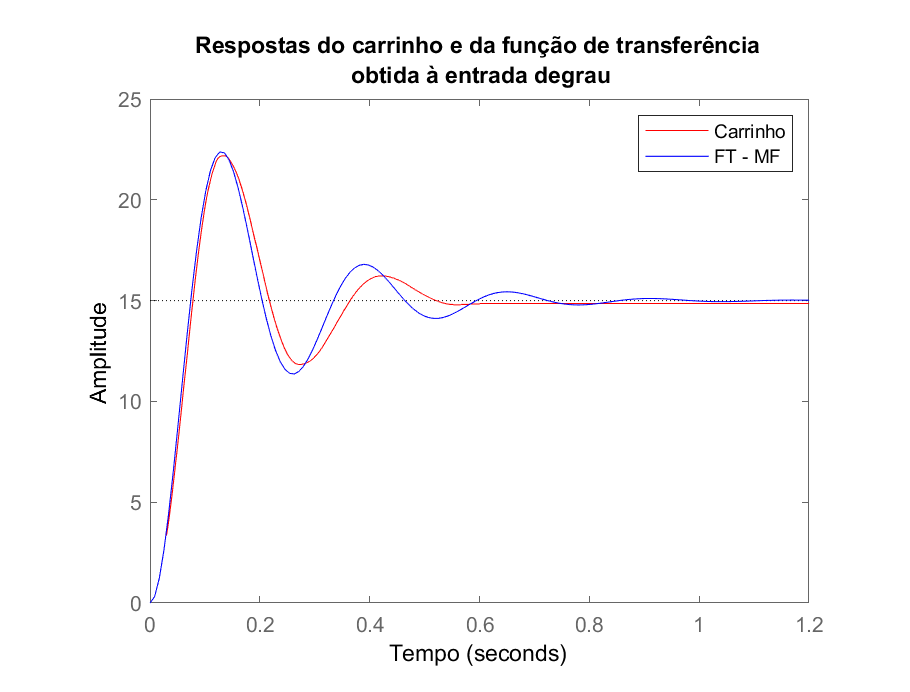
\includegraphics[width=.8\linewidth]{images/Matlab/identifica_01.eps}
        \caption{Comparação entre o resultado experiental e o modelo de segunda ordem.}\label{fig:resposta_modelo}
\end{figure}


\color{gray} \begin{verbatim}
a =
   10.8773

b =
  613.5793

k =
   2.5770e+05

g =
      613.6
  -------------
  s^2 + 10.88 s
 
Continuous-time transfer function.

gs =
          613.6
  ---------------------
  s^2 + 10.88 s + 613.6
 
Continuous-time transfer function.
\end{verbatim} \color{black}


\subsection{Discretização}

Após a definição do modelo dinâmico, a discretização do sistema por meio da transformada Z foi feita, seguindo o seguinte modelo da equação \ref{eq:trafoZ}.

\begin{equation}
    G(z) = (1-z^{-1}) \mathscr{Z}\left\{\frac{G(s)}{s}\right\}
    \label{eq:trafoZ}
\end{equation}

O \textit{script} de MATLAB equivalente pode ser observado a seguir

\begin{lstlisting}
ts = 0.05;                                  %Periodo de amostragem
discretizado = c2d(g, ts, 'zoh');           %discretizando a FT em malha aberta
[num, den] = tfdata(discretizado, 'v');     %obtendo os vetores de numerador e denominador
polos = roots(den);                         %obtendo o vetor de polos em Z
zeros = roots(num);                         %obtendo o vetor de zeros em Z
\end{lstlisting}

\color{gray} \begin{verbatim}
discretizado =
 
    0.645 z + 0.5382
  ---------------------
  z^2 - 1.58 z + 0.5805
 
Sample time: 0.05 seconds
Discrete-time transfer function.
\end{verbatim} \color{black}

\subsection{Requisitos}
{
    Para projetar o controlador, foram escolhidos o \textit{overshoot} e o tempo de acomodação desejados. A partir desses valores, o coeficiente de amortecimento e a frequência natural do projeto são calculados, e então é possível encontrar o polo em malha fechada desejado.
    
    O LGR do sistema discretizado com o polo em malha fechada é apresentado na Figura~\ref{fig:lgr_discreto}.
}

\begin{lstlisting}
MPreq = 0.2;            %overshoot máximo de 10%
TS2req = 0.3;           %tempo de acomodação (2%) máximo 0.5s

% Mp = exp ( (- pi * qsi) / sqrt( 1 - qsi^2 ) )
% qsi-req = abs(ln(Mp-req/100))/(sqrt(pi^2+ln(Mp-req/100)^2))
qsi_projeto = ( abs (log(MPreq/100)) / sqrt ((pi^2)+(log(MPreq/100)^2)) );

% Ts2= 4/(qsi*wn)
% wn-req = 4/(qsi-req*Ts2-req)
wn_projeto = 4/ (qsi_projeto * TS2req);

%polo desejado em Z
Zd = exp(-qsi_projeto * wn_projeto * ts) * exp (1j * sqrt(1-(qsi_projeto^2)) * wn_projeto * ts );

figure; rlocus (discretizado); hold on;
scatter (real(Zd),imag(Zd), 'filled');
\end{lstlisting}

\color{gray} \begin{verbatim}
qsi_projeto =
    0.8924

wn_projeto =
   14.9402

Zd =
   0.4845 + 0.1698i
\end{verbatim} \color{black}

\begin{figure}[H]
    \centering
        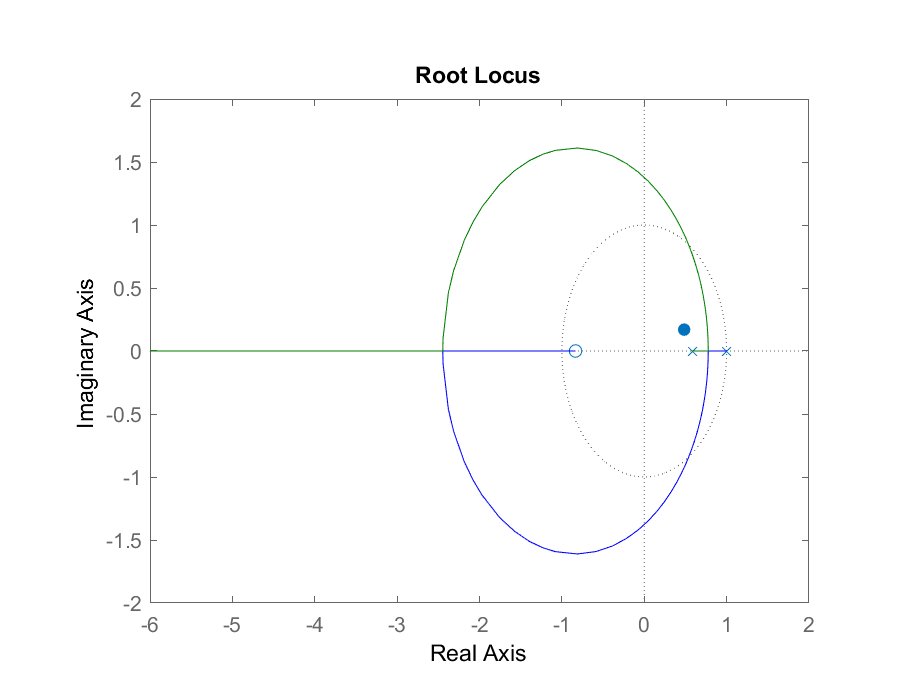
\includegraphics[width=.8\linewidth]{images/Matlab/identifica_02.eps}
        \caption{LGR do sistema discretizado.}\label{fig:lgr_discreto}
\end{figure}


\section{Projeto}

\subsection*{Controlador 1 - arbitrar zero com o mesmo valor da parte real dos polos desejados}

\begin{lstlisting}
G_Zd = polyval(num, Zd)/polyval(den, Zd);   %valor de G(Z_d)
phaseGZd = phase(G_Zd);                     %radianos
phaseGZddeg = rad2deg (phaseGZd);           %graus

phi = - pi - phaseGZd;              %radianos
phideg = rad2deg(phi);              %graus
phi360 = wrapTo360 (phideg);        %[0deg,360deg]

% parâmetros
a_proj1 = -real(Zd);
b_proj1 = -real(Zd) + (imag(Zd)*tan((pi/2) - phi));

% ganho
k_proj1 = abs(Zd + b_proj1) / ( abs(Zd + a_proj1)*abs(G_Zd) );

% controlador
Gd1 = zpk (-a_proj1,-b_proj1,k_proj1,ts);

% LGR
figure; rlocus (Gd1 * discretizado); hold on;
scatter (real(Zd),imag(Zd), 'filled');

% step
figure; plot(x(:,1),x(:,2),'r'); hold on; step(15 * gs, 'b'); step (15 * feedback(Gd1*discretizado, 1), 'g'); %step (15-(15*feedback(Gd1*discretizado,1))*Gd1,'y');
title({'Respostas do carrinho, sistema e sistema controlado','à entrada degrau'}); legend ('Carrinho', 'Sistema', 'Sistema controlado');
xlabel('Tempo');
\end{lstlisting}

\begin{figure}[H]
    \centering
        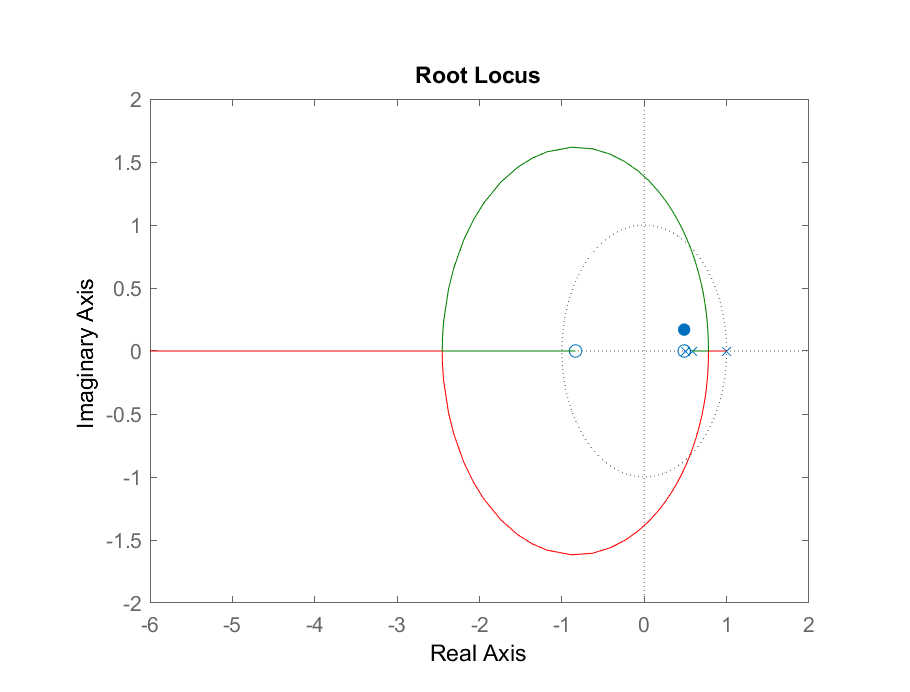
\includegraphics[width=.8\linewidth]{images/Matlab/identifica_03.eps}
        \caption{LGR do sistema.}\label{fig:lgr_controlador1}
\end{figure}
\begin{figure}[H]
    \centering
        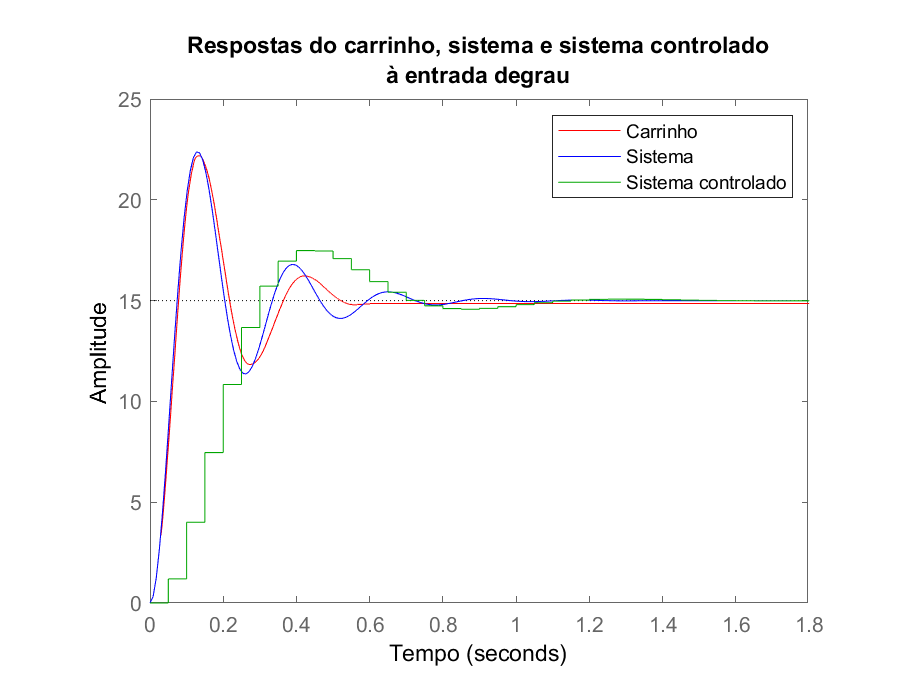
\includegraphics[width=.8\linewidth]{images/Matlab/identifica_04.eps}
        \caption{Resposta do sistema.}\label{fig:resposta_controlador1}
\end{figure}

\subsection*{Controlador 2 - utilizando a tática do triângulo isóceles:}

\begin{lstlisting}
% parâmetros
a_proj2 = - real(Zd) - imag(Zd)*tan((pi/2) - (phi/2));
b_proj2 = - real(Zd) + imag(Zd)*tan((pi/2) - (phi/2));

% ganho
k_proj2 = 1 / abs(G_Zd);

% controlador
Gd2 = zpk (-a_proj2,-b_proj2,k_proj2,ts);

% LGR
figure; rlocus (Gd2 * discretizado); hold on;
scatter (real(Zd),imag(Zd), 'filled');

%step
figure; plot(x(:,1),x(:,2),'r'); hold on; step(15 * gs, 'b'); step (15*feedback(Gd2*discretizado, 1), 'g'); %step (15-(15*feedback(Gd2*discretizado,1))*Gd2,'y');
title({'Respostas do carrinho, sistema e sistema controlado','à entrada degrau'}); legend ('Carrinho', 'Sistema', 'Sistema controlado');
xlabel('Tempo');
\end{lstlisting}

\begin{figure}[H]
    \centering
        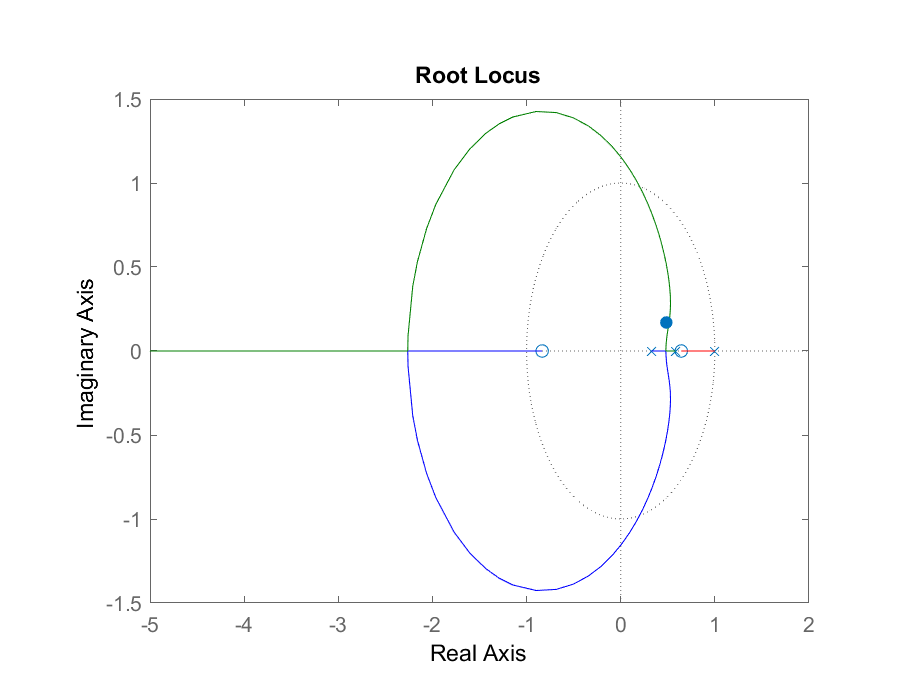
\includegraphics[width=.8\linewidth]{images/Matlab/identifica_05.eps}
        \caption{LGR do sistema.}\label{fig:lgr_controlador2}
\end{figure}
\begin{figure}[H]
    \centering
        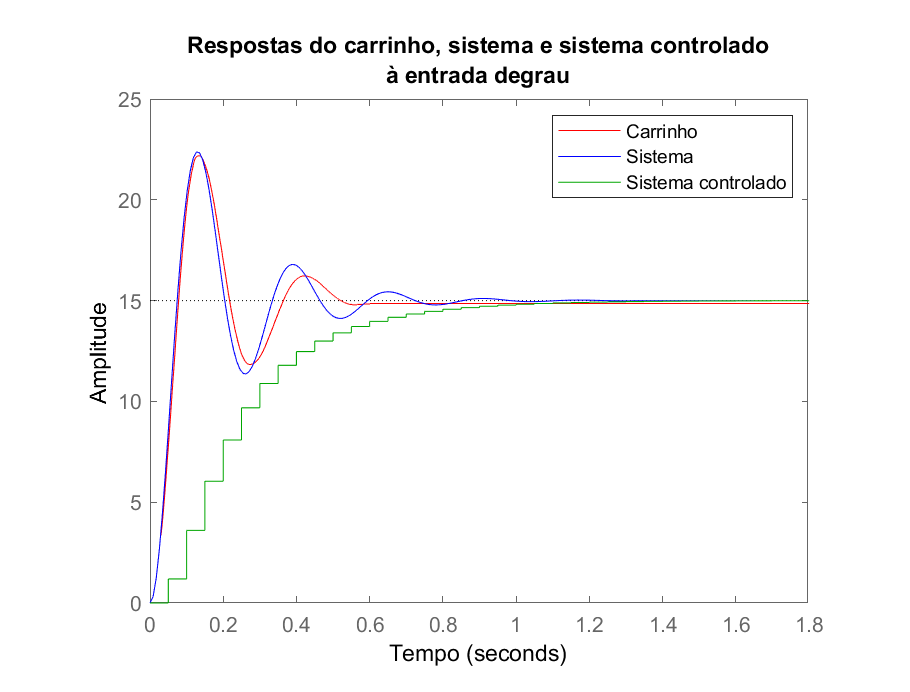
\includegraphics[width=.8\linewidth]{images/Matlab/identifica_06.eps}
        \caption{Resposta do sistema.}\label{fig:resposta_controlador2}
\end{figure}


\subsection*{Controlador 3 - cancelamento de polo}

\begin{lstlisting}
contrib_ang_zero = atan(imag(Zd)/(real(Zd)-zeros(1))); %radianos
contrib_ang_polo1 = atan(imag(Zd)/(real(Zd)-polos(1))); %radianos
contrib_ang_polo2 = atan(imag(Zd)/(real(Zd)-polos(2))); %radianos

soma_das_contrib_ang_em_zd = contrib_ang_zero - contrib_ang_polo1 - contrib_ang_polo2; %radianos
deficiencia_angular = soma_das_contrib_ang_em_zd - pi; %radianos


beta = tan(deficiencia_angular - contrib_ang_polo2)*imag(Zd);
k_gd = abs(Zd + beta) / ( abs(Zd + polos(2))*abs(G_Zd) );
g_d = zpk (polos(2), -beta, k_gd, ts);


% LGR
figure; rlocus (g_d * discretizado); hold on;
scatter (real(Zd),imag(Zd), 'filled');

%step
figure; plot(x(:,1),x(:,2),'r'); hold on; step(15 * gs, 'b'); step (15*feedback(g_d*discretizado, 1), 'g'); %step (15-(15*feedback(Gd2*discretizado,1))*Gd2,'y');
title({'Respostas do carrinho, sistema e sistema controlado','à entrada degrau'}); legend ('Carrinho', 'Sistema', 'Sistema controlado');
xlabel('Tempo');
\end{lstlisting}

\begin{figure}[H]
    \centering
        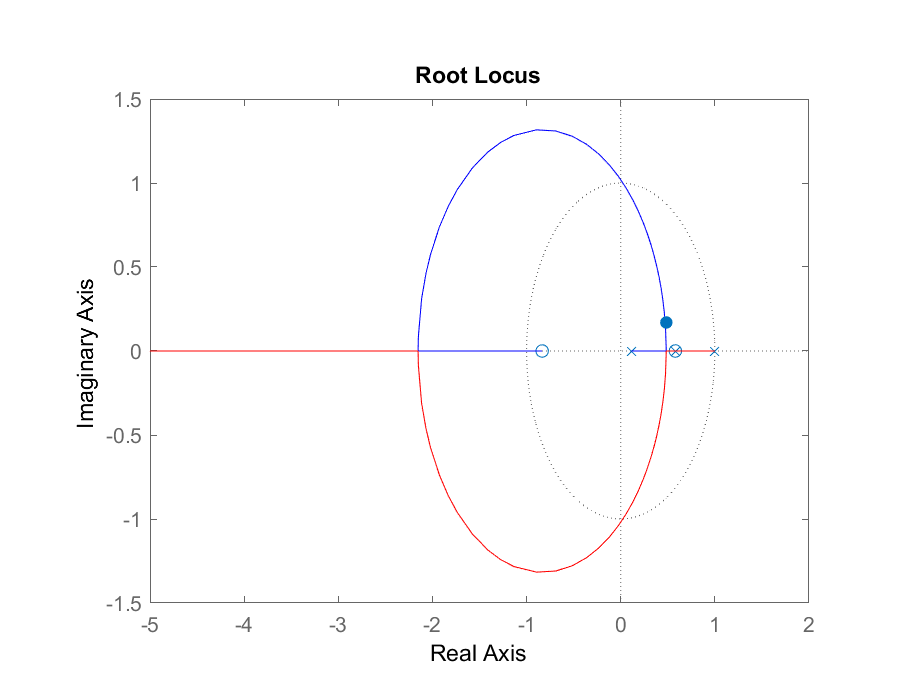
\includegraphics[width=.8\linewidth]{images/Matlab/identifica_07.eps}
        \caption{LGR do sistema.}\label{fig:lgr_controlador3}
\end{figure}
\begin{figure}[H]
    \centering
        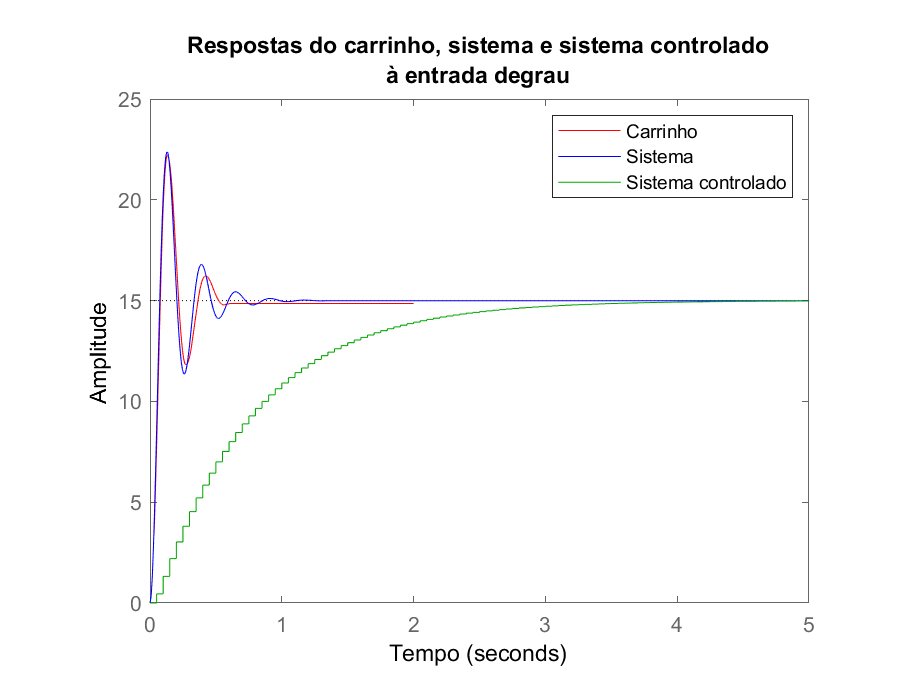
\includegraphics[width=.8\linewidth]{images/Matlab/identifica_08.eps}
        \caption{Resposta do sistema.}\label{fig:resposta_controlador3}
\end{figure}


\subsection{\textit{SISOTOOLS}}

Com o auxílio da ferramenta \textit{SISOTOOLS}, foi possível elaborar um quarto controlador, ajustando o polo e o zero manualmente para tentar obter uma resposta melhor do que os três métodos de controle apresentados acima.

\begin{figure}[H]
    \centering
        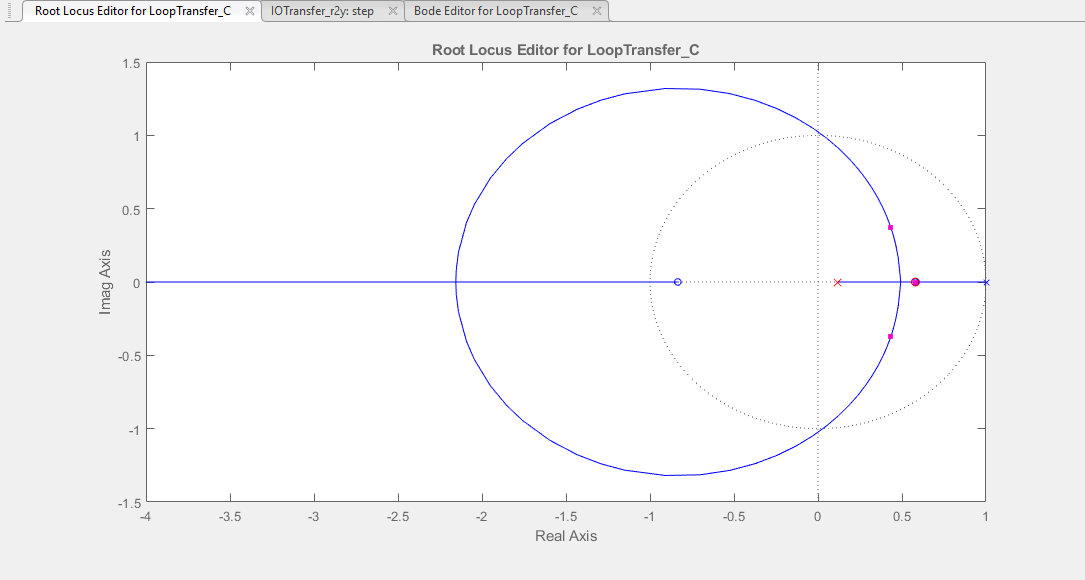
\includegraphics[width=.8\linewidth]{images/Matlab/SISOTOOLS-LGR.PNG}
        \caption{Definição de controlador usando o LGR usando a ferramenta \textit{SISOTOOLS}}\label{fig:SISOTOOLS-LGR}
\end{figure}

\begin{figure}[H]
    \centering
        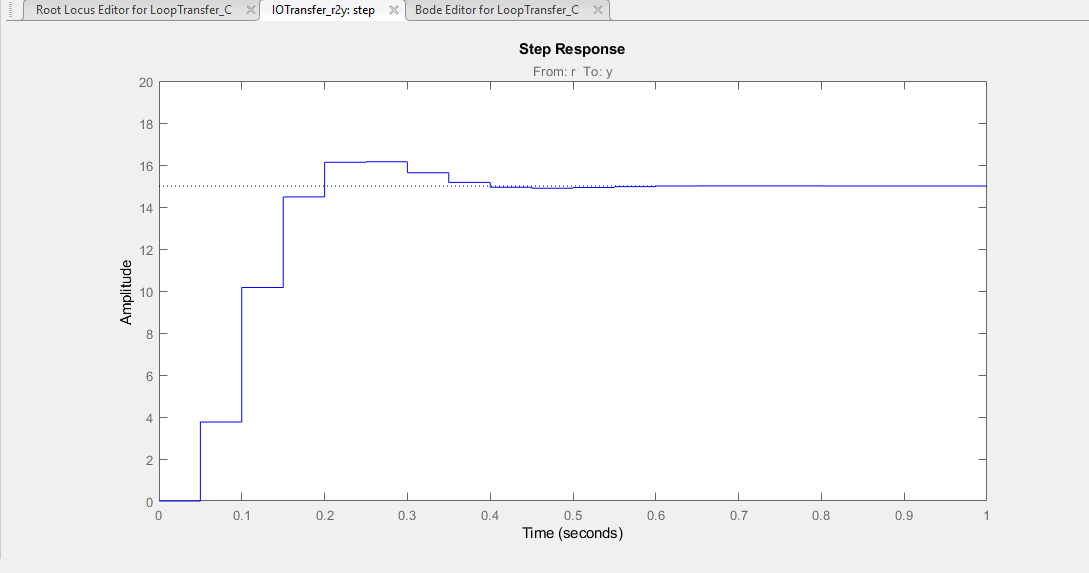
\includegraphics[width=.8\linewidth]{images/Matlab/SISOTOOLS-STEP.PNG}
        \caption{Resposta ao degrau da planta em malha fechada - controlador desenvolvido com a ferramenta  \textit{SISOTOOLS}}\label{fig:SISOTOOLS-STEP}
\end{figure}

\section{Resultados}

Em todos os quatro projetos de controlador, nenhuma resposta pode ser observada na planta durante a execução do experimento. Isso provavelmente decorre de um erro na modelagem que não conseguimos identificar.

Por um lado, durante o experimento na planta, o \textit{scope} do SIMULINK indicou que a ação de controle na entrada da planta era praticamente nula. Por outro, outro \textit{scope} mostrou um sinal saturado, oscilatório e de altíssima frequência, na saída do controlador. Nenhum dos dois casos condiz com as simulações feitas anteriormente.

\section{Conclusão}
{
    Não foi possível verificar na planta o funcionamento dos controladores projetados, porém o processo de elaboração de quatro controladores foi bastante instrutivo.
}

%\begin{figure}[H]
%    \centering
%        
\includegraphics[width=.8\linewidth]{deuces.jpg}
%        \caption{é nois}\label{ehnois}
%\end{figure}

\end{document}

% Referências
\bibliographystyle{abbrv}
\bibliography{references} % Acrescentadas no arquivo references.bib
% para usa-las no texto batsa usar \citep{} ou acrescentar diretamente usando \nocite{}
\nocite{resp-seg-ordem}
\nocite{req-temp-disc}
\nocite{proj-lgr}
\nocite{criterios-freq}
\nocite{proj-freq}